%
% $RCSfile: physical_architecture.tex,v $
%
% Copyright (c) 2001-2004. Christian Heller. All rights reserved.
%
% No copying, altering, distribution or any other actions concerning this
% document, except after explicit permission by the author!
% At some later point in time, this document is planned to be put under
% the GNU FDL license. For now, _everything_ is _restricted_ by the author.
%
% http://www.cybop.net
% - Cybernetics Oriented Programming -
%
% http://www.resmedicinae.org
% - Information in Medicine -
%
% @author Christian Heller <christian.heller@tuxtax.de>
%

\section{Physical Architecture}
\label{physical_architecture_heading}

This section wants to give practical proof of the theoretical models described
before. It first introduces the project \emph{Res Medicinae} in whose frame the
software was written. Afterwards, two solutions of a physical architecture,
\emph{Two-Tier} and \emph{Three-Tier} are explained.

%
% $RCSfile: res_medicinae.tex,v $
%
% Copyright (C) 2002-2008. Christian Heller.
%
% Permission is granted to copy, distribute and/or modify this document
% under the terms of the GNU Free Documentation License, Version 1.1 or
% any later version published by the Free Software Foundation; with no
% Invariant Sections, with no Front-Cover Texts and with no Back-Cover
% Texts. A copy of the license is included in the section entitled
% "GNU Free Documentation License".
%
% http://www.cybop.net
% - Cybernetics Oriented Programming -
%
% http://www.resmedicinae.org
% - Information in Medicine -
%
% Version: $Revision: 1.1 $ $Date: 2008-08-19 20:41:08 $ $Author: christian $
% Authors: Christian Heller <christian.heller@tuxtax.de>
%

\chapter{Res Medicinae}
\label{res_medicinae_heading}
\index{Res Medicinae Application Prototype}

\begin{flushright}
    \textsl{
        No Road can ever be too long,\\
        side-by-side with a good Friend.
    }\\
    \textsc{Unknown Author}
\end{flushright}

The first two chapters (\ref{cybernetics_oriented_language_heading} and
\ref{cybernetics_oriented_interpreter_heading}) of part \ref{proof_heading} of
this work defined the CYBOL language and its corresponding interpreter CYBOI.
Since a theory is worth more if it can be proven in practice, this chapter will
describe an effort trying to apply both to create an application system named
\emph{Res Medicinae} \cite{resmedicinae} (Latin for \emph{Matter of Medicine}).

%
% $RCSfile: project.tex,v $
%
% Copyright (C) 2002-2008. Christian Heller.
%
% Permission is granted to copy, distribute and/or modify this document
% under the terms of the GNU Free Documentation License, Version 1.1 or
% any later version published by the Free Software Foundation; with no
% Invariant Sections, with no Front-Cover Texts and with no Back-Cover
% Texts. A copy of the license is included in the section entitled
% "GNU Free Documentation License".
%
% http://www.cybop.net
% - Cybernetics Oriented Programming -
%
% http://www.resmedicinae.org
% - Information in Medicine -
%
% Version: $Revision: 1.1 $ $Date: 2008-08-19 20:41:08 $ $Author: christian $
% Authors: Christian Heller <christian.heller@tuxtax.de>
%

\section{Project}
\label{project_heading}
\index{Res Medicinae Project}
\index{Hospital Information System}
\index{HIS}
\index{Practice Management System}
\index{PMS}
\index{Electronic Health Record}
\index{EHR}

The -- somewhat idealistic -- aim was initially to create the prototype of a
\emph{Hospital Information System} (HIS). Due to the clearly too high-set aims,
this was later revised so that the focus of the prototype became a standard
\emph{Practice Management System} (PMS) with an \emph{Electronic Health Record}
(EHR) as its core. Several technology changes during the progress of this work
and the lack in time required to also revise this aim, so that now the final
prototype consists of just the (rudimentary) address management module of the
planned EHR application. It is written in CYBOL and executable by CYBOI.

The following sections describe the project background of \emph{Res Medicinae}.

%
% $RCSfile: free_and_open_source_software.tex,v $
%
% Copyright (C) 2002-2008. Christian Heller.
%
% Permission is granted to copy, distribute and/or modify this document
% under the terms of the GNU Free Documentation License, Version 1.1 or
% any later version published by the Free Software Foundation; with no
% Invariant Sections, with no Front-Cover Texts and with no Back-Cover
% Texts. A copy of the license is included in the section entitled
% "GNU Free Documentation License".
%
% http://www.cybop.net
% - Cybernetics Oriented Programming -
%
% http://www.resmedicinae.org
% - Information in Medicine -
%
% Version: $Revision: 1.1 $ $Date: 2008-08-19 20:41:06 $ $Author: christian $
% Authors: Christian Heller <christian.heller@tuxtax.de>
%

\subsection{Free and Open Source Software}
\label{free_and_open_source_software_heading}
\index{Free and Open Source Software}
\index{FOSS}
\index{Free/ Libre Open Source Software}
\index{FLOSS}
\index{General Public License}
\index{GPL}
\index{Free Documentation License}
\index{FDL}
\index{Open Source Software}
\index{OSS}

Just like CYBOP (including CYBOL and CYBOI) \cite{cybop}, \emph{Res Medicinae}
\cite{resmedicinae} is developed within a \emph{Free/ Libre Open Source Software}
(FLOSS) project. Its source code, resources and documentation are placed under
GNU's \emph{General Public License} (GPL) (section
\ref{gnu_general_public_license_heading}) and \emph{Free Documentation License}
(FDL) (section \ref{gnu_free_documentation_license_heading}), respectively.
That means they can be freely redistributed and modified under the terms of
these licences. Although distributed in the hope that they will be useful, the
program and its resources come \emph{without any warranty}, without even the
implied warranty of \emph{merchantability or fitness for a particular purpose}.
See \cite{gnulicences} for details.

More information on \emph{Open Source Software} (OSS) in general can be found
at \cite{opensource}. There are plenty of resources for further background
reading, a German one being the \emph{Open Source Jahrbuch 2004}
\cite{opensourcejahrbuch2004}. To what concerns FLOSS in the medical arena,
many other projects exist. Comprehensive lists of these can be found at
\cite{euspirit, linuxmednews, medhowto}.

%
% $RCSfile: portals_and_services.tex,v $
%
% Copyright (C) 2002-2008. Christian Heller.
%
% Permission is granted to copy, distribute and/or modify this document
% under the terms of the GNU Free Documentation License, Version 1.1 or
% any later version published by the Free Software Foundation; with no
% Invariant Sections, with no Front-Cover Texts and with no Back-Cover
% Texts. A copy of the license is included in the section entitled
% "GNU Free Documentation License".
%
% http://www.cybop.net
% - Cybernetics Oriented Programming -
%
% http://www.resmedicinae.org
% - Information in Medicine -
%
% Version: $Revision: 1.1 $ $Date: 2008-08-19 20:41:08 $ $Author: christian $
% Authors: Christian Heller <christian.heller@tuxtax.de>
%

\subsection{Portals and Services}
\label{portals_and_services_heading}
\index{Open Source Development Portals and Services}
\index{Sourceforge Development Portal}
\index{Freshmeat Development Portal}
\index{BerliOS Development Portal}
\index{Savannah Development Portal}
\index{Free Software Foundation}
\index{FSF}

As OSS became popular over the years, the number of its supporters rose. It is
not long time that \emph{Sourceforge} \cite{sourceforge}, the first
\emph{Development Portal} for FLOSS, was opened. Shortly after, others like
\emph{Freshmeat} \cite{freshmeat} followed and meanwhile, there are also
national initiatives like \emph{BerliOS} \cite{berlios} in Germany. Also the
\emph{Free Software Foundation} (FSF) offers an own portal called
\emph{Savannah} \cite{savannah}, hosting exclusively \emph{free} \cite{gnu}
software projects. Figure \ref{portals_figure} shows the four portals by their
name, logo and \emph{Uniform Resource Locator} (URL).

\begin{figure}[ht]
    \begin{center}
        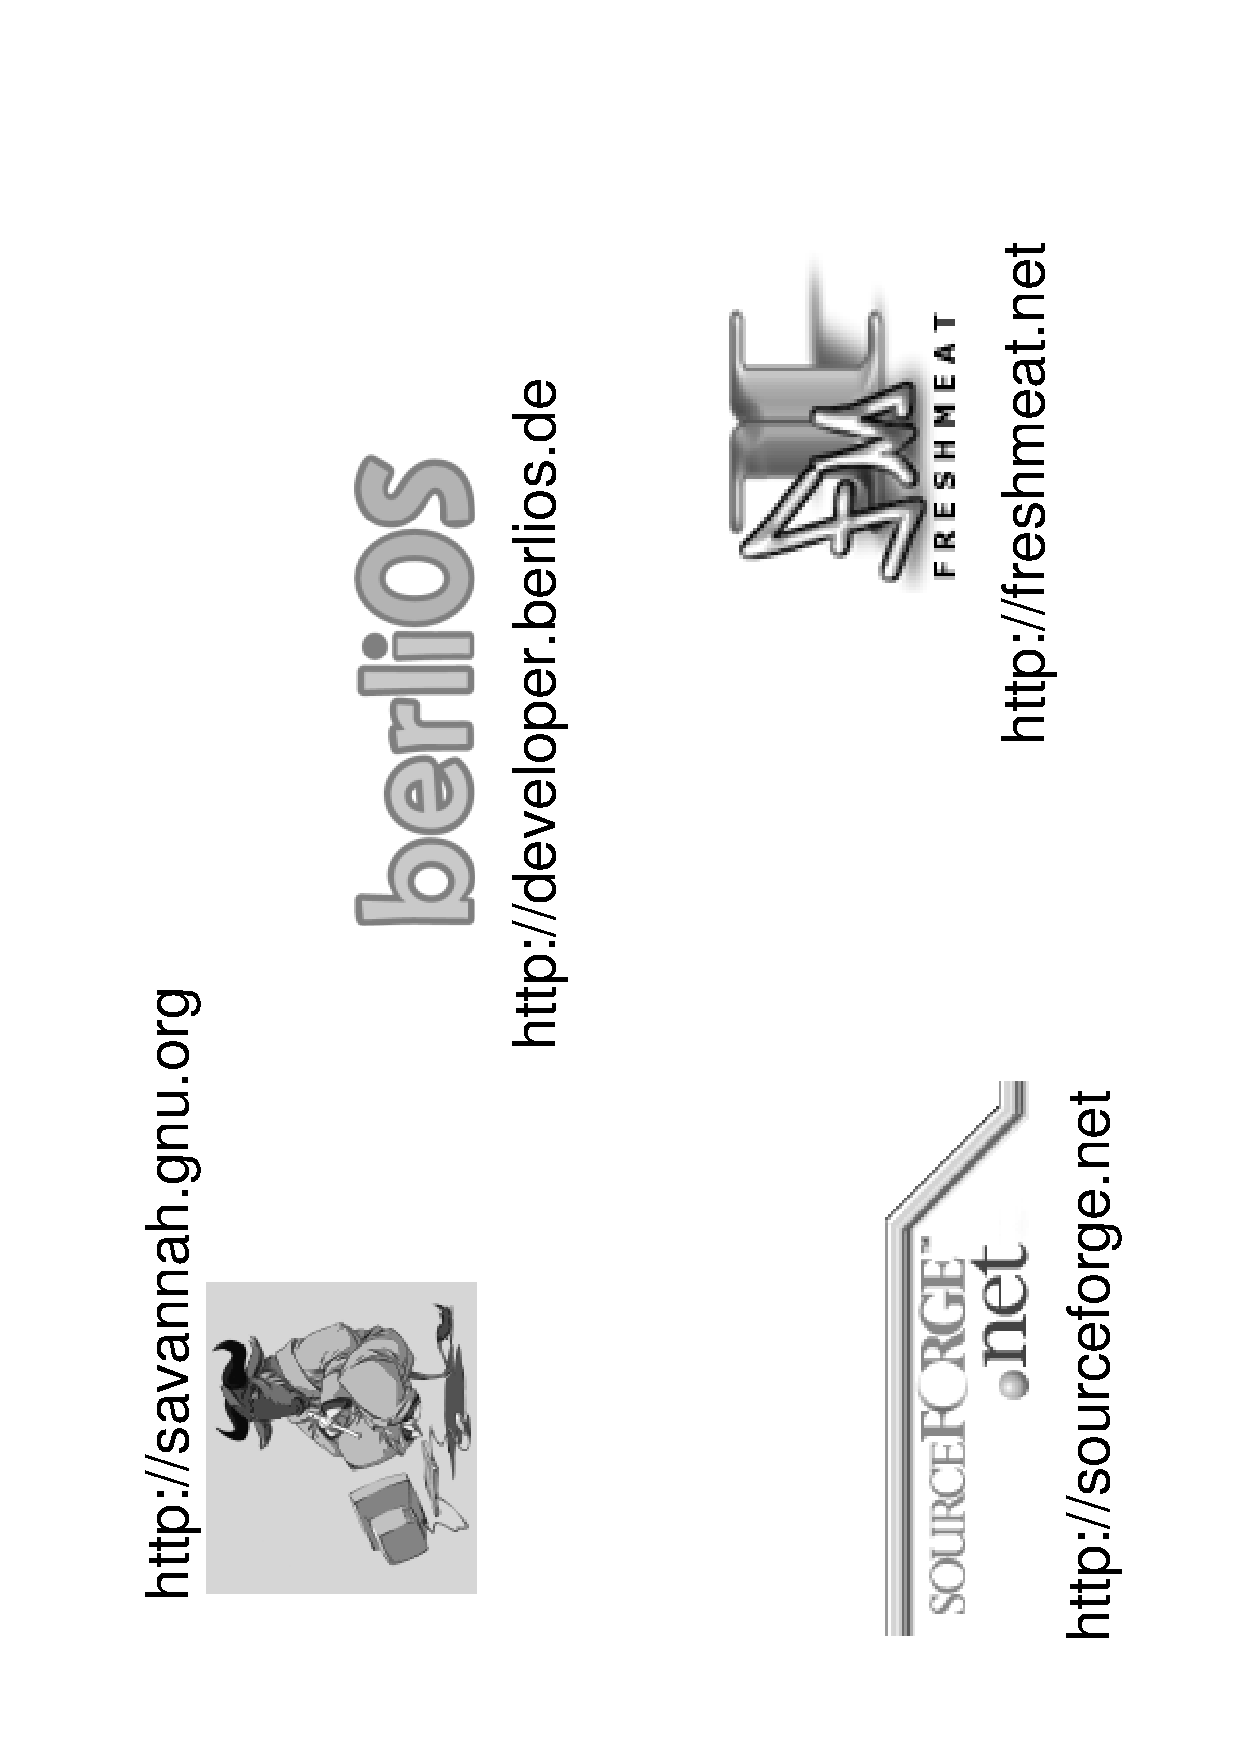
\includegraphics[scale=0.3,angle=-90]{graphic/portals.pdf}
        \caption{FLOSS Development Portals}
        \label{portals_figure}
    \end{center}
\end{figure}

As \emph{BerliOS} states in its slogan, it is the aim of development portals of
that kind to \textit{foster open source development}. In \emph{Savannah's}
words, they are \textit{central points for the development, distribution and
maintenance of FLOSS}. Although very often supported by well-known sponsors,
most portals are and want to stay independent. Using them, OSS projects and their
developers are offered several free services (figure \ref{services_figure}).
Since not all of these are always useful, projects can configure their portal
sites as needed.

\begin{figure}[ht]
    \begin{center}
        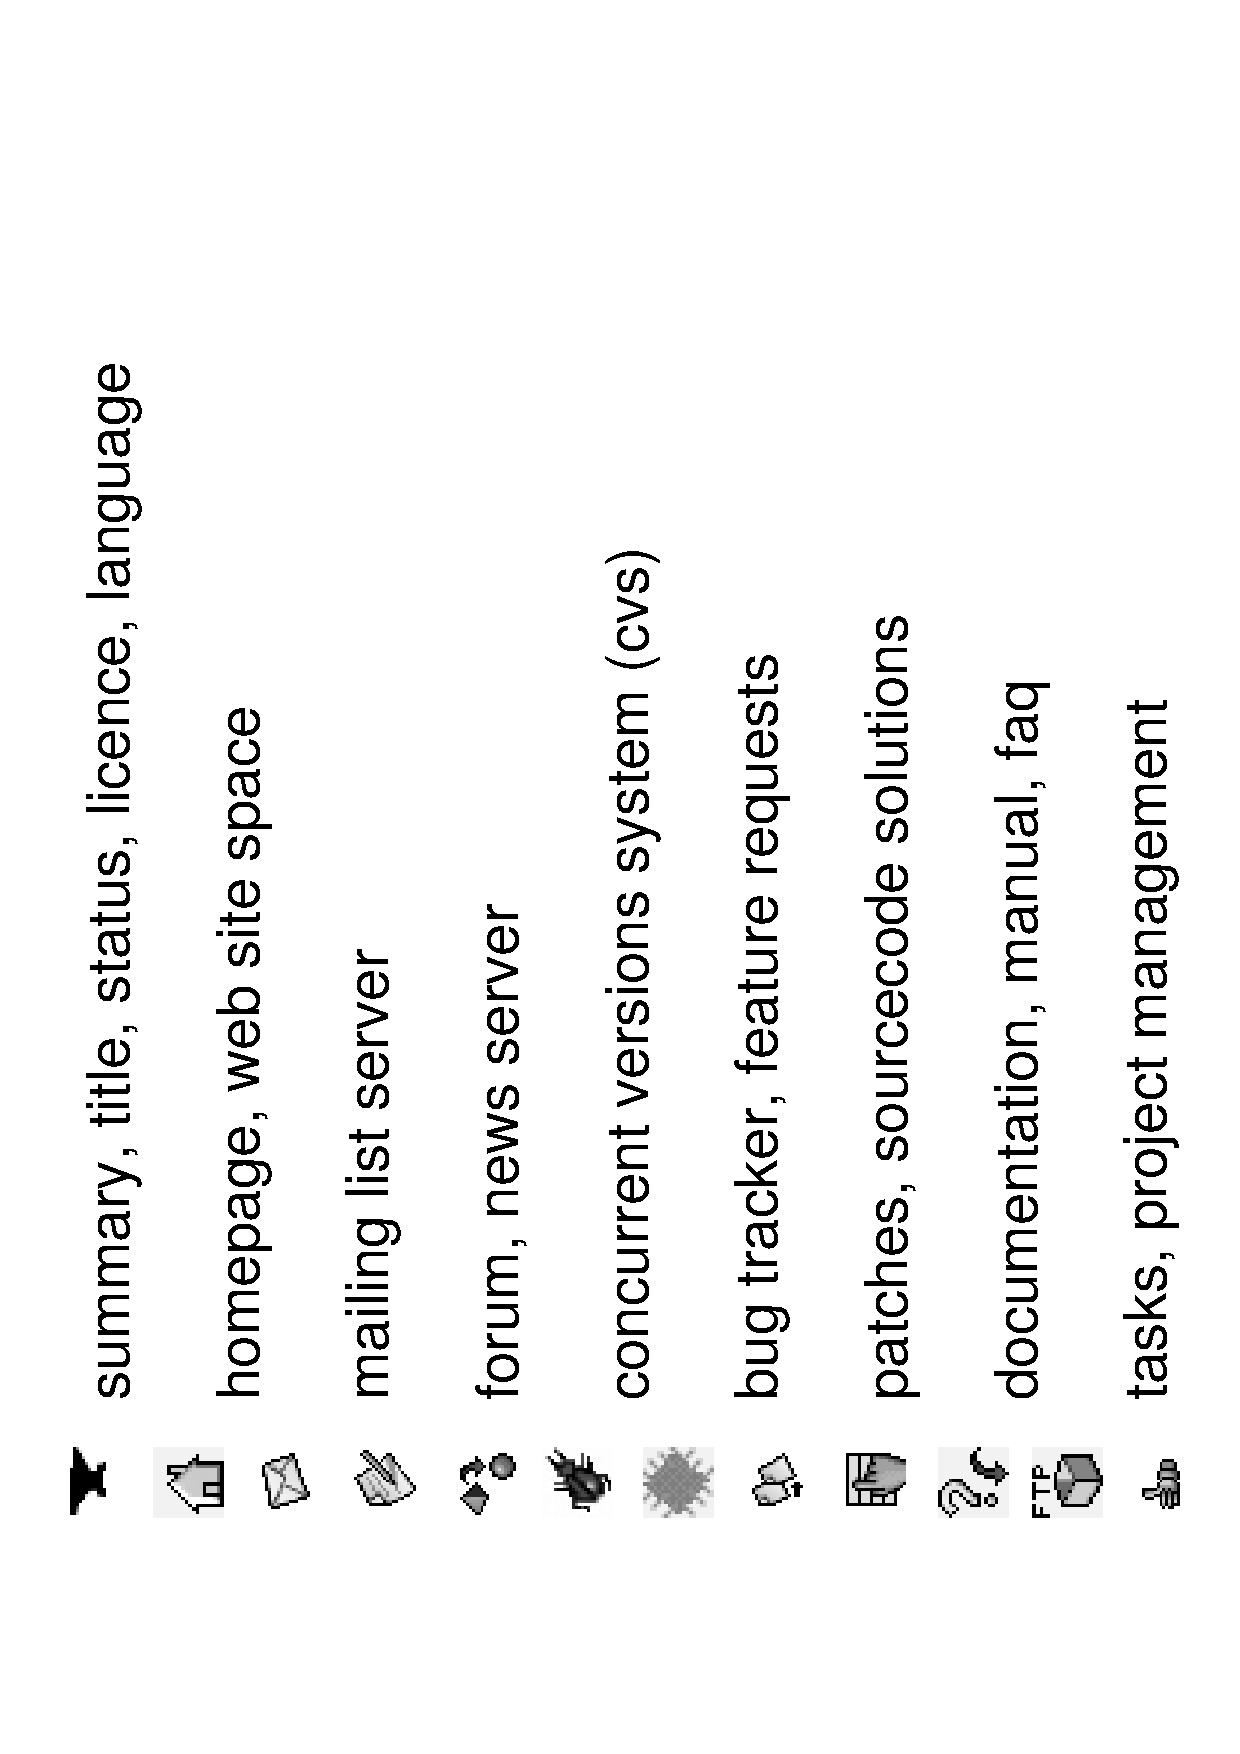
\includegraphics[scale=0.3,angle=-90]{graphic/services.pdf}
        \caption{Portal Services}
        \label{services_figure}
    \end{center}
\end{figure}

\emph{Res Medicinae} was one of the first OSS projects registered at
Sourceforge (number 4237 of now more than 100,000). CYBOP (CYBOL, CYBOI) is
hosted at BerliOS.

%
% $RCSfile: tools.tex,v $
%
% Copyright (C) 2002-2008. Christian Heller.
%
% Permission is granted to copy, distribute and/or modify this document
% under the terms of the GNU Free Documentation License, Version 1.1 or
% any later version published by the Free Software Foundation; with no
% Invariant Sections, with no Front-Cover Texts and with no Back-Cover
% Texts. A copy of the license is included in the section entitled
% "GNU Free Documentation License".
%
% http://www.cybop.net
% - Cybernetics Oriented Programming -
%
% http://www.resmedicinae.org
% - Information in Medicine -
%
% Version: $Revision: 1.1 $ $Date: 2008-08-19 20:41:09 $ $Author: christian $
% Authors: Christian Heller <christian.heller@tuxtax.de>
%

\subsection{Tools}
\label{tools_heading}
\index{Res Medicinae Development Tools}

Classical application development relies on tools like a \emph{UML Designer}, for
creating \emph{Unified Modeling Language} (UML) diagrams, a \emph{Text Editor},
\emph{Compiler} and \emph{Debugger}. Nowadays, these and other tools are
offered in one package, as \emph{Integrated Development Environment} (IDE).

Because the CYBOI interpreter is written in the system programming language
\emph{C}, its development requires a compiler. CYBOL applications, on the other
hand, do not have to be compiled. They base on interpreted XML code which can
be written in every text editor; nothing else is needed. An adapted editor was
proposed in section \ref{template_editor_heading}.

Res Medicinae development could certainly be speeded up by using graphical
diagrams in the style of the UML. But unfortunately, design tools that directly
support CYBOP do not exist yet. As section \ref{knowledge_designer_heading}
tried to show, some UML diagrams could be used with only minor adaptations for
CYBOL modelling. For the time being, standard XML editors have to suffice.

For running and testing CYBOL applications, of course, the CYBOI interpreter is
needed.

%
% $RCSfile: contributors.tex,v $
%
% Copyright (C) 2002-2008. Christian Heller.
%
% Permission is granted to copy, distribute and/or modify this document
% under the terms of the GNU Free Documentation License, Version 1.1 or
% any later version published by the Free Software Foundation; with no
% Invariant Sections, with no Front-Cover Texts and with no Back-Cover
% Texts. A copy of the license is included in the section entitled
% "GNU Free Documentation License".
%
% http://www.cybop.net
% - Cybernetics Oriented Programming -
%
% http://www.resmedicinae.org
% - Information in Medicine -
%
% Version: $Revision: 1.1 $ $Date: 2008-08-19 20:41:06 $ $Author: christian $
% Authors: Christian Heller <christian.heller@tuxtax.de>
%

\subsection{Contributors}
\label{contributors_heading}
\index{Res Medicinae Contributors}
\index{Open Source Health Care Alliance}
\index{OSHCA}

OSS projects are not only \emph{Hobby Activities} any longer. Many of them have
long overtaken their commercial competitors, in functionality, stability,
security and popularity. Due to the participation of sometimes hundreds of
enthusiasts, they mostly have much greater momentum.

In the case of \emph{Res Medicinae}, a number of \emph{Medical Doctors} (MD)
and \emph{Software Engineers} have contributed with their work or expressed
serious interest in collaboration. Many \emph{Informatics Students} were (and
are) involved and completed their diploma (master) works on a topic within the
project. Finally, there are the OSS projects that follow similar aims, like:

\begin{itemize}
    \item[-] \emph{GNUmed} \cite{gnumed}
    \item[-] \emph{Open Source Clinical Application Resource} (OSCAR) \cite{oscar}
    \item[-] \emph{Care2002} (Care2x) \cite{care2x}
    \item[-] \emph{Torch} \cite{torch}
    \item[-] \emph{Open Infrastructure for Outcomes} (OIO) \cite{oio}
    \item[-] \emph{Veterans Health Information Systems and Technology Architecture} (VistA) \cite{vista}
    \item[-] \emph{OpenEMed} \cite{openemed}
    \item[-] \emph{Tcl/Tk Family Practice} (tkFP) \cite{openehr}
    \item[-] \emph{Debian-Med} \cite{debianmed}, as meta project for packaging
\end{itemize}

All of them want to provide software solutions for medicine. Being friendly
concurrents, they use mailing lists such as \cite{openhealth} to exchange
latest insights, offer help to each other and work towards a better integration.
The technological decisions that have originally caused a division of forces
and a multitude of projects to exist, may in the end turn out to be fruitful,
with focus on the interoperability of systems. Additionally, organisations like
the \emph{Open Source Health Care Alliance} (OSHCA) \cite{oshca} bundle the
projects' forces and regularly organise conferences.


%
% $RCSfile: analysis.tex,v $
%
% Copyright (C) 2002-2008. Christian Heller.
%
% Permission is granted to copy, distribute and/or modify this document
% under the terms of the GNU Free Documentation License, Version 1.1 or
% any later version published by the Free Software Foundation; with no
% Invariant Sections, with no Front-Cover Texts and with no Back-Cover
% Texts. A copy of the license is included in the section entitled
% "GNU Free Documentation License".
%
% http://www.cybop.net
% - Cybernetics Oriented Programming -
%
% http://www.resmedicinae.org
% - Information in Medicine -
%
% Version: $Revision: 1.1 $ $Date: 2008-08-19 20:41:05 $ $Author: christian $
% Authors: Christian Heller <christian.heller@tuxtax.de>
%

\section{Analysis}
\label{analysis_heading}
\index{Res Medicinae Requirements Analysis}
\index{Software Engineering Process}
\index{SEP}
\index{Electronic Health Record}
\index{EHR}

Abiding by the standard \emph{Software Engineering Process} (SEP) (chapter
\ref{software_engineering_process_heading}), a \emph{Requirements Analysis}
stood as first activity for the development of \emph{Res Medicinae}. The
following sections will give a brief overview of some requirements and current
modelling trends, concerning the \emph{Electronic Health Record} (EHR). They do
\emph{not} try to replace more comprehensive works written on the subject.

%
% $RCSfile: requirements_document.tex,v $
%
% Copyright (C) 2002-2008. Christian Heller.
%
% Permission is granted to copy, distribute and/or modify this document
% under the terms of the GNU Free Documentation License, Version 1.1 or
% any later version published by the Free Software Foundation; with no
% Invariant Sections, with no Front-Cover Texts and with no Back-Cover
% Texts. A copy of the license is included in the section entitled
% "GNU Free Documentation License".
%
% http://www.cybop.net
% - Cybernetics Oriented Programming -
%
% http://www.resmedicinae.org
% - Information in Medicine -
%
% Version: $Revision: 1.1 $ $Date: 2008-08-19 20:41:08 $ $Author: christian $
% Authors: Christian Heller <christian.heller@tuxtax.de>
%

\subsection{Requirements Document}
\label{requirements_document_heading}
\index{Res Medicinae Requirements Document}
\index{DocBook DTD}
\index{The Linux Documentation Project}
\index{TLDP}

With the help of German medical doctors, a \emph{Requirements Document}
\cite{resmedicinae2001} was created and is meanwhile being updated and extended
since about five years. It basically describes an EHR and the information it
should include.

Since the document itself is just a hierarchical model consisting of parts, it
can well be represented in CYBOL. Unfortunately, a document processor that can
read and render CYBOL, in the style of \emph{LaTeX} \cite{latex}, has not been
written to date (although CYBOI might integrate this functionality one day). It
was therefore decided to write the requirements document in SGML/ XML, using
the \emph{DocBook} DTD \cite{docbook} and tools described in
\emph{The Linux Documentation Project} (TLDP) \cite{linuxdoc}.

%
% $RCSfile: ehr_and_co.tex,v $
%
% Copyright (C) 2002-2008. Christian Heller.
%
% Permission is granted to copy, distribute and/or modify this document
% under the terms of the GNU Free Documentation License, Version 1.1 or
% any later version published by the Free Software Foundation; with no
% Invariant Sections, with no Front-Cover Texts and with no Back-Cover
% Texts. A copy of the license is included in the section entitled
% "GNU Free Documentation License".
%
% http://www.cybop.net
% - Cybernetics Oriented Programming -
%
% http://www.resmedicinae.org
% - Information in Medicine -
%
% Version: $Revision: 1.1 $ $Date: 2008-08-19 20:41:06 $ $Author: christian $
% Authors: Christian Heller <christian.heller@tuxtax.de>
%

\subsection{EHR \& Co.}
\label{ehr_and_co_heading}
\index{Electronic Health Record}
\index{EHR}
\index{Personal Health Record}
\index{PHR}
\index{Virtual Health Record}
\index{VHR}
\index{Virtual Patient Record}
\index{VPR}
\index{Electronic Medical Record}
\index{EMR}
\index{Electronic Patient Record}
\index{EPR}
\index{Computer-based Patient Record}
\index{CPR}
\index{Computerised Patient Record}
\index{CPR}
\index{Computerised Medical Record}
\index{CMR}
\index{Automated Medical Record}
\index{AMR}
\index{Digital Medical Record}
\index{DMR}
\index{Patient Carried Record}
\index{PCR}
\index{Patient Medical Record}
\index{PMR}
\index{Integrated Care Record}
\index{ICR}
\index{Electronic Medical Infrastructure}
\index{EMI}
\index{Lifetime Data Repository}
\index{LDR}

Besides the now quite common term \emph{Electronic Health Record} (EHR), some
publications, experts or companies also talk of \cite{marietti, waegemann}:

\begin{itemize}
    \item[-] \emph{Personal Health Record} (PHR)
    \item[-] \emph{Virtual Health Record} (VHR)
    \item[-] \emph{Virtual Patient Record} (VPR)
    \item[-] \emph{Electronic Medical Record} (EMR)
    \item[-] \emph{Electronic Patient Record} (EPR)
    \item[-] \emph{Computer-based Patient Record} (CPR)
    \item[-] \emph{Computerised Patient Record} (CPR)
    \item[-] \emph{Computerised Medical Record} (CMR)
    \item[-] \emph{Automated Medical Record} (AMR)
    \item[-] \emph{Digital Medical Record} (DMR)
    \item[-] \emph{Patient Carried Record} (PCR)
    \item[-] \emph{Patient Medical Record} (PMR)
    \item[-] \emph{Integrated Care Record} (ICR)
    \item[-] \emph{Electronic Medical Infrastructure} (EMI)
    \item[-] \emph{Lifetime Data Repository} (LDR)
\end{itemize}

and state differences in their contents, access, maintainer, place of storage,
technology or other aspects. David Kibbe, for example, as cited by Jennifer
Bush \cite{bush}, says:

\begin{quote}
    There's recently been a subtle shift in terminology. EMR connotes a tool
    that's for doctors only and something that replaces the paper record with a
    database. EHR connotes more of a connectivity tool that not only includes
    the patient and may even be used by the patient, but also provides a set of
    tools to improve work-flow efficiency and quality of care in doctors' offices.

    \ldots\ An EHR should include a detailed clinical documentation function;
    prescription ordering and management capabilities; a secure messaging
    system; lab and test result reporting functions; evidence-based health
    guidelines; secure patient access to health records; a public health
    reporting- and tracking system; mapping to clinical- and standard code sets
    and the ability to interface with leading practice management software.
\end{quote}

In essence, however, most of the above-listed terms are considered synonymous,
since their definitions, if existent at all, differ just in nuances. Charlene
Marietti, who investigated in this subject, writes \cite{marietti}:

\begin{quote}
    Meanwhile, most practical people don't see a big difference between the CPR
    and the EMR and the many other terms that exist.
\end{quote}

Therefore, this work further on sticks to the term \emph{EHR} and wants it
understood as general description for either of the other terms mentioned
above.

%
% $RCSfile: episode_based.tex,v $
%
% Copyright (C) 2002-2008. Christian Heller.
%
% Permission is granted to copy, distribute and/or modify this document
% under the terms of the GNU Free Documentation License, Version 1.1 or
% any later version published by the Free Software Foundation; with no
% Invariant Sections, with no Front-Cover Texts and with no Back-Cover
% Texts. A copy of the license is included in the section entitled
% "GNU Free Documentation License".
%
% http://www.cybop.net
% - Cybernetics Oriented Programming -
%
% http://www.resmedicinae.org
% - Information in Medicine -
%
% Version: $Revision: 1.1 $ $Date: 2008-08-19 20:41:06 $ $Author: christian $
% Authors: Christian Heller <christian.heller@tuxtax.de>
%

\subsection{Episode Based}
\label{episode_based_heading}
\index{Episode Based EHR}
\index{Patient Centered Medical Record}
\index{Health Issue of an Episode Based EHR}
\index{Clinical Episode of an Episode Based EHR}
\index{Clinical Encounter of an Episode Based EHR}
\index{Clinical Item of an Episode Based EHR}
\index{Partial Contact of an Episode Based EHR}
\index{Problem Oriented Medical Record}
\index{POMR}

Historically, it took a long time until the concept of a modern EHR crystalised
out. An early form of a time-oriented medical record stems from Hippocrates
(5th century BC) who wanted to accurately reflect the course of a disease and
indicate its possible causes. In 1907, the \emph{Mayo Clinic} (formed by the
American surgeon William Mayo) adopted one separate file for each patient, to
be able to obtain a better overview of his complete disease history. This
innovation was the origin of the \emph{Patient Centered Medical Record} as
known today, as \cite{mihandbook} means.

The discussion on how to model an ideal EHR already lasts for decades and has
not finished. Recent proposals brought in some new perspectives and ideas. One
of them turns around the so-called \emph{Episode-based} EHR \cite{westerhof}.
In the centre of these considerations stands a structure that is described in a
more pragmatic way by Karsten Hilbert of GNUmed \cite{gnumed}. He sees a
complex EHR as hierarchical composition of the following items:

\begin{itemize}
    \item[-] Health Issue
    \item[-] Clinical Episode
    \item[-] Clinical Encounter
    \item[-] Clinical Item
\end{itemize}

The additional concept of a \emph{Partial Contact} as known from the Dutch
\emph{Episode Model} does not integrate into this hierarchy. But after Hilbert,
\emph{Partial Contacts} could be easily derived from existing EHR data by
aggregating all \emph{Clinical Items} that belong to the same
\emph{Clinical Encounter} and the same \emph{Clinical Episode}.

\emph{Clinical Items} are typically elements in the \emph{SOAP} format of
progress notes, as known from the \emph{Problem Oriented Medical Record} (POMR)
\cite{weed} that was introduced by Lawrence L. Weed in the 1960s. SOAP stands
for:

\begin{itemize}
    \item[-] \emph{Subjective:} Complaints as phrased by the patient
    \item[-] \emph{Objective:} Findings of physicians and nurses
    \item[-] \emph{Assessment:} Test results and conclusions, such as a diagnosis
    \item[-] \emph{Plan:} Medical plan, for example treatment or policy
\end{itemize}

%
% $RCSfile: evidence_based.tex,v $
%
% Copyright (C) 2002-2008. Christian Heller.
%
% Permission is granted to copy, distribute and/or modify this document
% under the terms of the GNU Free Documentation License, Version 1.1 or
% any later version published by the Free Software Foundation; with no
% Invariant Sections, with no Front-Cover Texts and with no Back-Cover
% Texts. A copy of the license is included in the section entitled
% "GNU Free Documentation License".
%
% http://www.cybop.net
% - Cybernetics Oriented Programming -
%
% http://www.resmedicinae.org
% - Information in Medicine -
%
% Version: $Revision: 1.1 $ $Date: 2008-08-19 20:41:06 $ $Author: christian $
% Authors: Christian Heller <christian.heller@tuxtax.de>
%

\subsection{Evidence Based}
\label{evidence_based_heading}
\index{Evidence Based EHR}
\index{Virtual Record (EHR)}

In an email to the \emph{Open Health Mailing List} \cite{openhealth}, David R.
raised a number of unsolved issues concerning the \emph{Evidence-based} EHR.
In a first thought, he exposes the existence of two distinct views on an EHR:
\emph{clinical} and \emph{evidential}. A medical record were not just a
collection of clinical information, but also a \emph{Legal Document} with
financial importance. It were to give evidence of the healthcare services
rendered by a particular provider for a particular organisation, and the reason
why, mostly, patients do not own the record. Finally, an EHR were the result of
the intersection of two major business processes: the \emph{Clinical Process}
and the \emph{Records Management Process}.

This observation leads to the second important question whether records should
be \emph{accessed} remotely, leaving them in place at each of the organisations
where the patient has been seen, or be \emph{incorporated} as extract or full
copy to each organisation's repository, as known from the paper-based world.
Since the first method, promoted as trans-organisational \emph{Virtual Record},
did not address an organisation's need for maintaining its evidential records,
it had, in the opinion of David R., failed to gain widespread or long-term
acceptance.

A third point turns around the authoring of an EHR. Record keeping were no
longer simply a \emph{personal} activity but rather an \emph{inter-personal}
action. David R. writes on:

\begin{quote}
    Historically, providers have viewed the medical records they have created
    as though they were a personal journal kept by the provider to facilitate
    his or her process of delivering care to an individual patient. It was
    viewed as an aid to memory and extended the provider's thought across time.
    \ldots\ In the setting of a highly mobile population of patients and
    providers, the record becomes a living document with multiple authors.
    Multiple individuals for multiple reasons consult it and \ldots\ it is in
    this record that a shared understanding of the (health) problems and
    recommended solutions for \ldots\ the individual occur.
\end{quote}

Because the EHR could be seen as a space for collaboration, applications
working with it had to support clinical process \emph{Workflow} requirements. A
new set of demands were also placed on health care providers, to document their
activities with patients in a way that is mutually \emph{intelligible} to those
who have a stake in the information contained in the record.

%
% $RCSfile: continuity_of_care.tex,v $
%
% Copyright (C) 2002-2008. Christian Heller.
%
% Permission is granted to copy, distribute and/or modify this document
% under the terms of the GNU Free Documentation License, Version 1.1 or
% any later version published by the Free Software Foundation; with no
% Invariant Sections, with no Front-Cover Texts and with no Back-Cover
% Texts. A copy of the license is included in the section entitled
% "GNU Free Documentation License".
%
% http://www.cybop.net
% - Cybernetics Oriented Programming -
%
% http://www.resmedicinae.org
% - Information in Medicine -
%
% Version: $Revision: 1.1 $ $Date: 2008-08-19 20:41:06 $ $Author: christian $
% Authors: Christian Heller <christian.heller@tuxtax.de>
%

\subsection{Continuity of Care}
\label{continuity_of_care_heading}
\index{Continuity of Care Record}
\index{CCR}
\index{Personal Health Project}
\index{PHP}

A main result of the opinion stated in the previous section was the realisation
that a major challenge for EHR design will be to overcome the difference
between an organisation's evidential record management process with emphasis on
\emph{legal/ financial aspects} and the record keeping as
\emph{medical/ health documentation}, that an individual would do.

This is exactly the issue that Philippe Ameline and his French colleagues
address in their \emph{Nautilus/ Odyssee} project \cite{nautilus}. It
distinguishes between three levels of data:

\begin{itemize}
    \item[-] \emph{Individual}: personal, various local
    \item[-] \emph{Group}: professional, 24 hour availability
    \item[-] \emph{Collective}: dedicated to continuity of care
\end{itemize}

The latter is called \emph{Personal Health Project} (PHP). Its health management
data can be shared between a \emph{Patient} and his \emph{Care Team}, with the
EHR \emph{passing by} institutions. Ameline writes in \cite{openehrtechnical}
that the management of these two referentials -- health professional and patient
-- meant that applications now had to handle differently the \emph{history data}
with a time duration (which may get changed by someone else) and the data of the
\emph{instantaneous picture} kind (what one noticed and reported at a given time).

A similar effort with U.S. American roots is called \emph{Continuity of Care Record}
(CCR) \cite{ccr}. Just like the PHP, it does not want to be a complete EHR, but
rather: \textit{organise and make transportable a set of basic patient
information consisting of the most relevant and timely facts about a patient's
condition.} Through specified XML code, the CCR becomes interoperable.

%
% $RCSfile: core_model.tex,v $
%
% Copyright (C) 2002-2008. Christian Heller.
%
% Permission is granted to copy, distribute and/or modify this document
% under the terms of the GNU Free Documentation License, Version 1.1 or
% any later version published by the Free Software Foundation; with no
% Invariant Sections, with no Front-Cover Texts and with no Back-Cover
% Texts. A copy of the license is included in the section entitled
% "GNU Free Documentation License".
%
% http://www.cybop.net
% - Cybernetics Oriented Programming -
%
% http://www.resmedicinae.org
% - Information in Medicine -
%
% Version: $Revision: 1.1 $ $Date: 2008-08-19 20:41:06 $ $Author: christian $
% Authors: Christian Heller <christian.heller@tuxtax.de>
%

\subsection{Core Model}
\label{core_model_heading}
\index{Res Medicinae Core Model}
\index{Electronic Health Record as Core Model}

Many kinds of application modules are needed in a healthcare-specific
\emph{Information Technology} (IT) environment. The tasks they fulfill,
together with a proposed name within the \emph{Res Medicinae} project, are
listed following:

\begin{itemize}
    \item[-] \emph{Revue:} Portal for module starting
    \item[-] \emph{Residenz:} Administrative data management
    \item[-] \emph{Record:} Clinical documentation
    \item[-] \emph{Rezept:} Prescription ordering and management
    \item[-] \emph{Reform:} Form printing
    \item[-] \emph{Report:} Public health reporting and tracking
    \item[-] \emph{Reagenz:} Laboratory- and test result retrieval
    \item[-] \emph{Rendezvous:} Scheduling
    \item[-] \emph{Roentgen:} Clinical imaging
    \item[-] \emph{Rechnung:} Billing
    \item[-] \emph{Richtig:} Statistics
    \item[-] \emph{Register:} Pharmaceutical reference
    \item[-] \emph{Ratlos:} Lexicon-, terminology- and code set query
\end{itemize}

\begin{figure}[ht]
    \begin{center}
        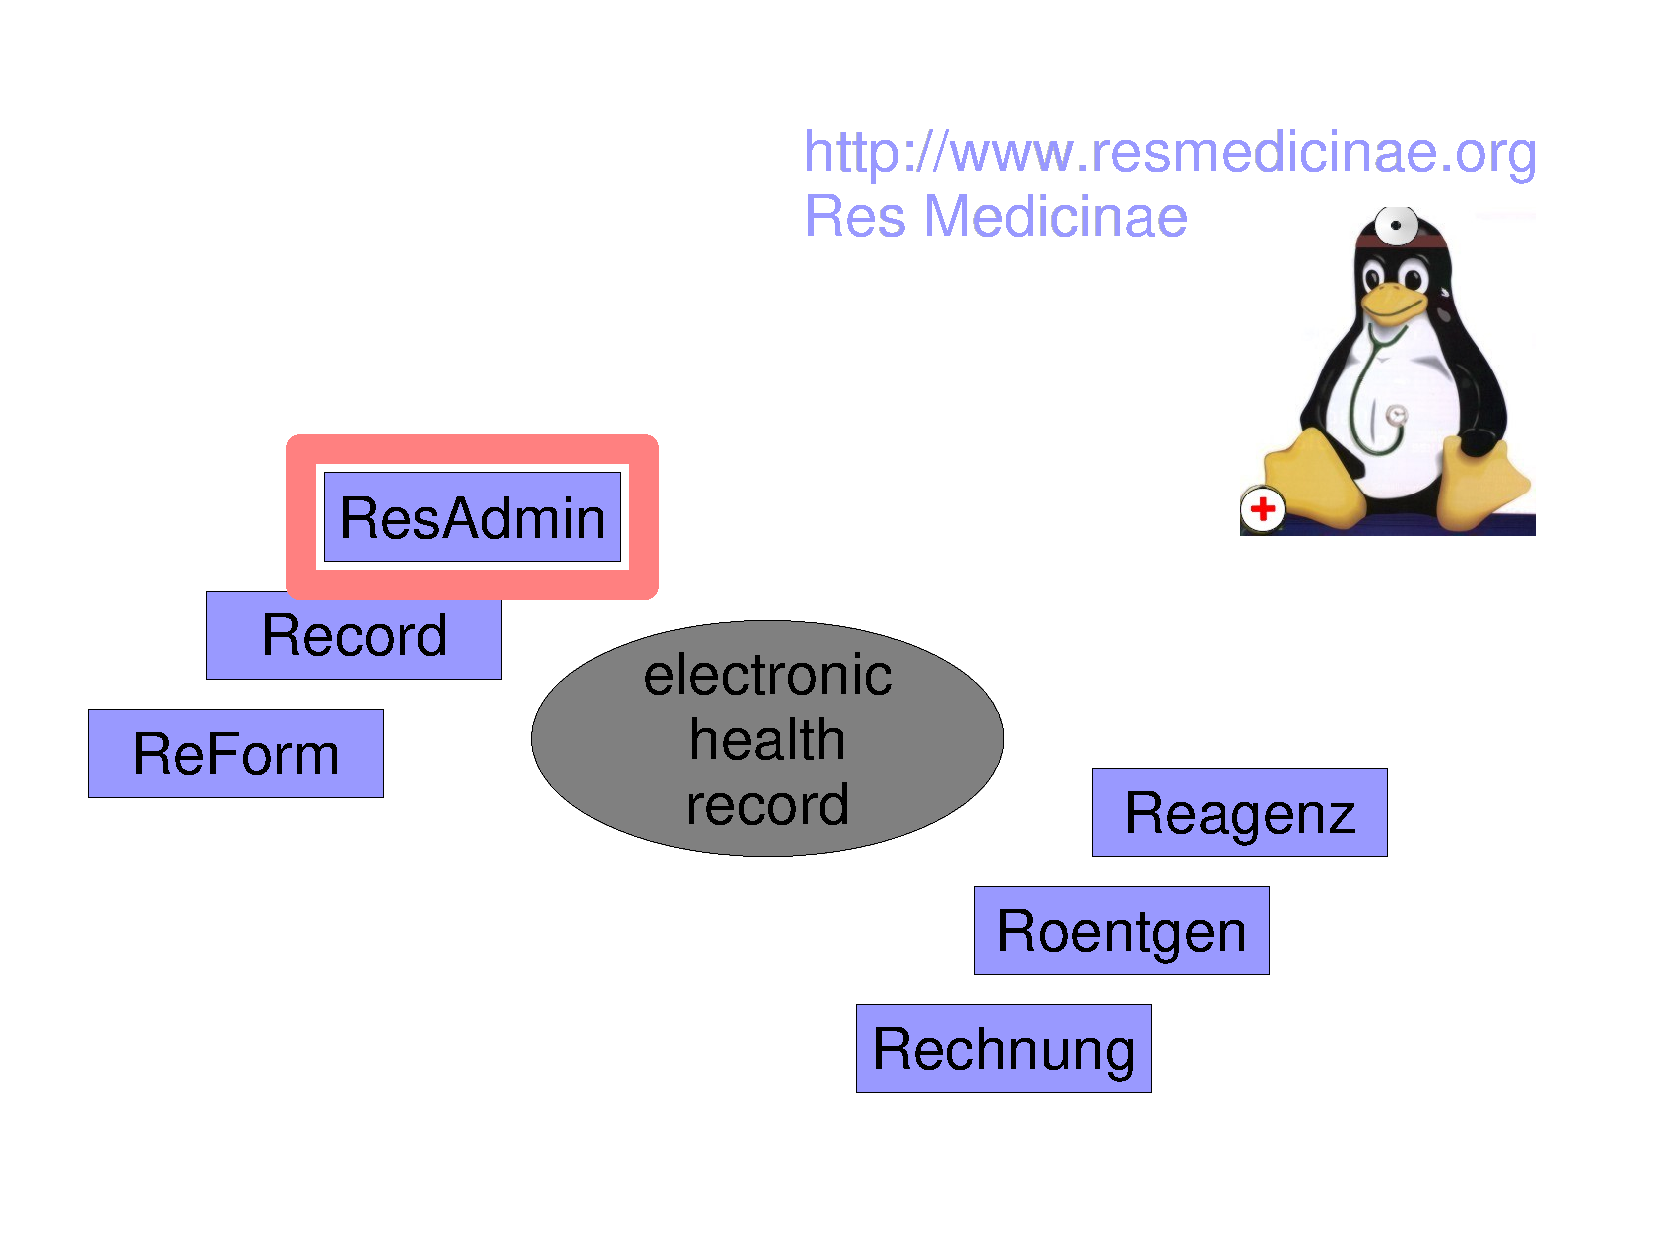
\includegraphics[scale=0.3,angle=-90]{graphic/core.pdf}
        \caption{Applications Grouped around an Electronic Health Record Core}
        \label{core_figure}
    \end{center}
\end{figure}

Figure \ref{core_figure} shows some of these modules, together with an EHR as
their central data structure.


\newpage
%
% $RCSfile: standards.tex,v $
%
% Copyright (C) 2002-2008. Christian Heller.
%
% Permission is granted to copy, distribute and/or modify this document
% under the terms of the GNU Free Documentation License, Version 1.1 or
% any later version published by the Free Software Foundation; with no
% Invariant Sections, with no Front-Cover Texts and with no Back-Cover
% Texts. A copy of the license is included in the section entitled
% "GNU Free Documentation License".
%
% http://www.cybop.net
% - Cybernetics Oriented Programming -
%
% http://www.resmedicinae.org
% - Information in Medicine -
%
% Version: $Revision: 1.1 $ $Date: 2008-08-19 20:41:09 $ $Author: christian $
% Authors: Christian Heller <christian.heller@tuxtax.de>
%

\section{Standards}
\label{standards_heading}
\index{Medical Informatics Standards}

In a further thought, current standards of medical informatics had to be
considered for the development of \emph{Res Medicinae} application modules.
There exists a whole plethora of (partly \emph{de facto}) standards -- far too
many to discuss here. The following sections will give a brief overview of only
a few standards which are potentially important for EHR development.

%
% $RCSfile: overview.tex,v $
%
% Copyright (C) 2002-2008. Christian Heller.
%
% Permission is granted to copy, distribute and/or modify this document
% under the terms of the GNU Free Documentation License, Version 1.1 or
% any later version published by the Free Software Foundation; with no
% Invariant Sections, with no Front-Cover Texts and with no Back-Cover
% Texts. A copy of the license is included in the section entitled
% "GNU Free Documentation License".
%
% http://www.cybop.net
% - Cybernetics Oriented Programming -
%
% http://www.resmedicinae.org
% - Information in Medicine -
%
% Version: $Revision: 1.1 $ $Date: 2008-08-19 20:41:08 $ $Author: christian $
% Authors: Christian Heller <christian.heller@tuxtax.de>
%

\subsection{Overview}
\label{overview_heading}
\index{Medical Informatics Working Groups}
\index{Deutsches Institut fuer Normung}
\index{DIN}
\index{Comite Europeen de Normalisation}
\index{CEN}
\index{International Organization for Standardization}
\index{ISO}

Figure \ref{groups_figure} shows the medical informatics working groups of
important standardisation organisations, namely the:

\begin{itemize}
    \item[-] \emph{Deutsches Institut fuer Normung} (DIN)
    \item[-] \emph{Comite Europeen de Normalisation} (CEN)
    \item[-] \emph{International Organization for Standardization} (ISO)
\end{itemize}

\begin{figure}[ht]
    \begin{center}
        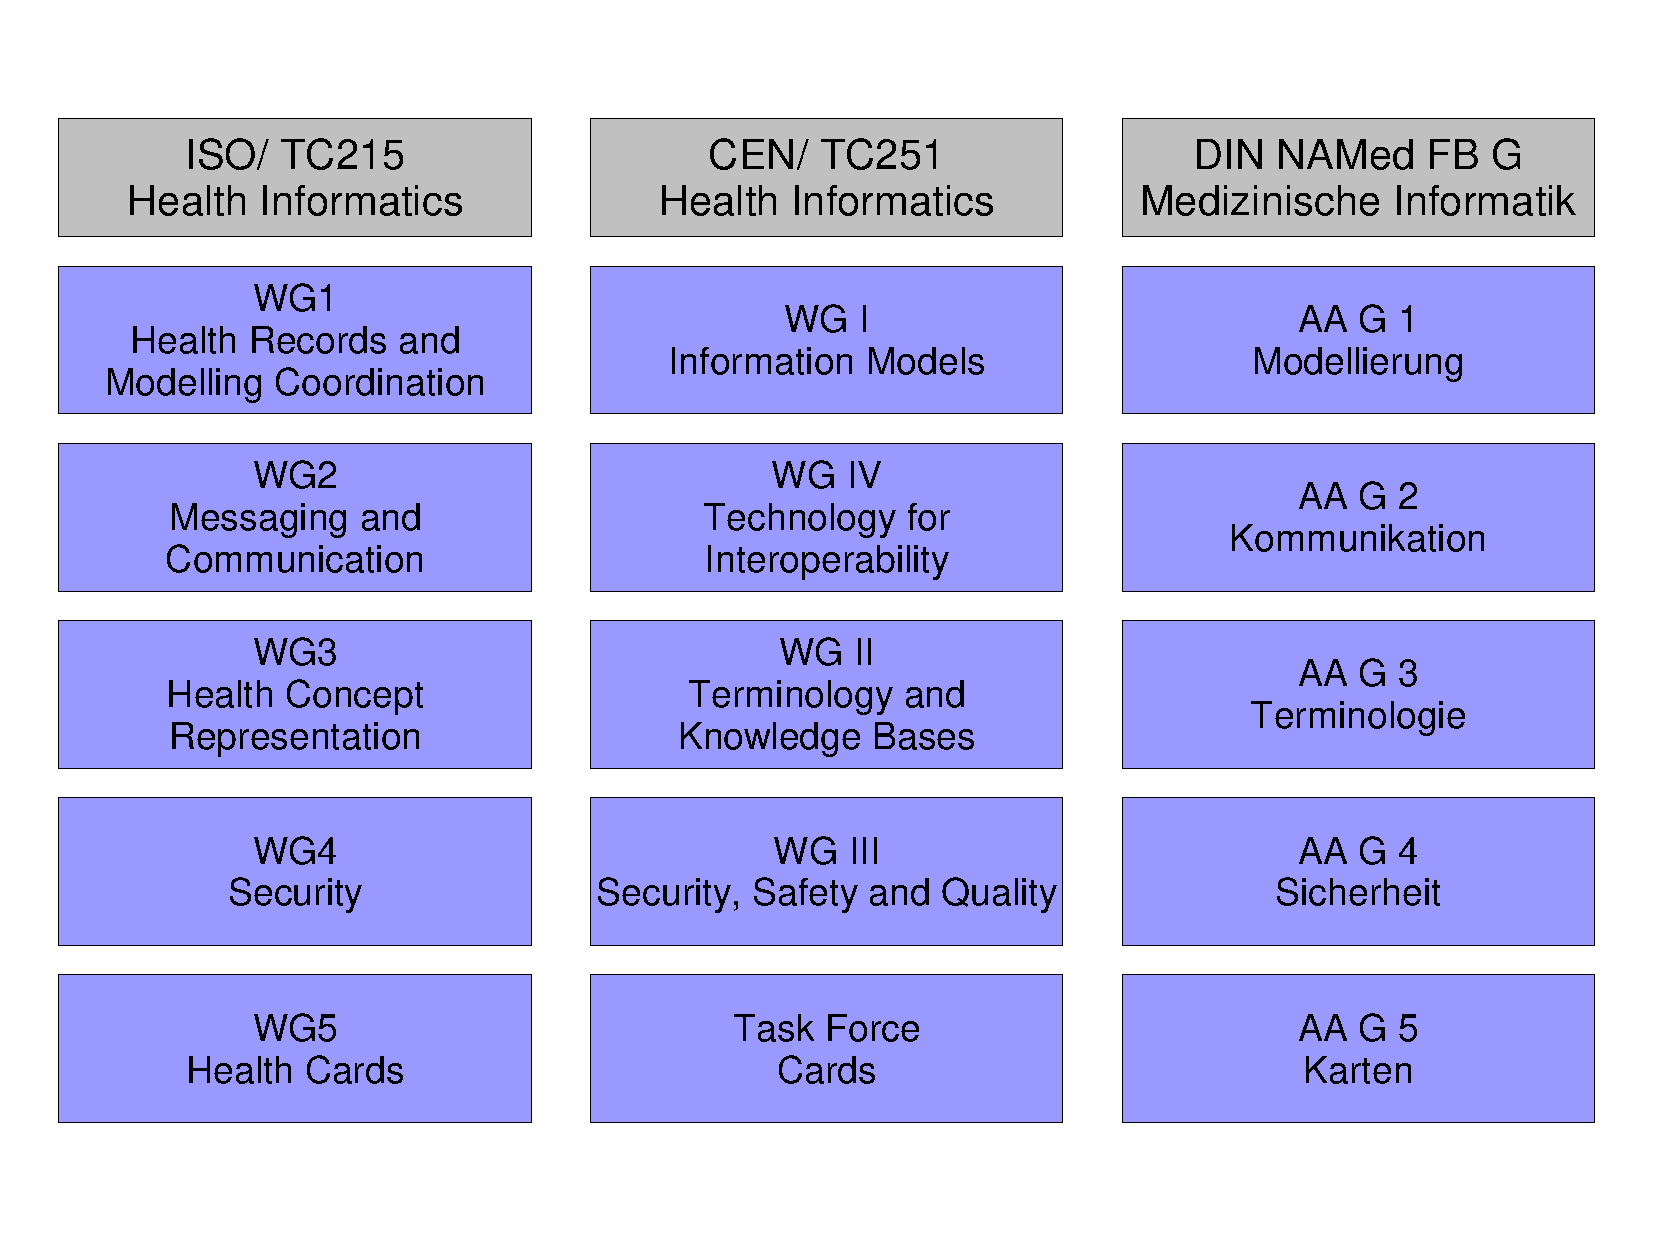
\includegraphics[scale=0.3,angle=-90]{graphic/groups.pdf}
        \caption{Medical Informatics Working Groups of DIN/ CEN/ ISO \cite{atgexpertsreport}}
        \label{groups_figure}
    \end{center}
\end{figure}

The structure of the following sections is chosen after this systematics.
Standards for \emph{Health Record Modelling} will be described first, followed
by those for \emph{Messaging and Communication} and a section on
\emph{Terminology- and Coding Systems}. \emph{Imaging-}, \emph{Health Card-}
and further standards are mentioned afterwards. General remarks on current
\emph{Standards Development Processes} follow. Reflections on the
\emph{Implications} of standards on the development of \emph{Res Medicinae}
will conclude the topic.

%
% $RCSfile: record_modelling.tex,v $
%
% Copyright (C) 2002-2008. Christian Heller.
%
% Permission is granted to copy, distribute and/or modify this document
% under the terms of the GNU Free Documentation License, Version 1.1 or
% any later version published by the Free Software Foundation; with no
% Invariant Sections, with no Front-Cover Texts and with no Back-Cover
% Texts. A copy of the license is included in the section entitled
% "GNU Free Documentation License".
%
% http://www.cybop.net
% - Cybernetics Oriented Programming -
%
% http://www.resmedicinae.org
% - Information in Medicine -
%
% Version: $Revision: 1.1 $ $Date: 2008-08-19 20:41:08 $ $Author: christian $
% Authors: Christian Heller <christian.heller@tuxtax.de>
%

\subsection{Record Modelling}
\label{record_modelling_heading}
\index{Medical Record Modelling Standards}

\input{cen_tc251}
\input{open_ehr}

%
% $RCSfile: messaging_and_communication.tex,v $
%
% Copyright (C) 2002-2008. Christian Heller.
%
% Permission is granted to copy, distribute and/or modify this document
% under the terms of the GNU Free Documentation License, Version 1.1 or
% any later version published by the Free Software Foundation; with no
% Invariant Sections, with no Front-Cover Texts and with no Back-Cover
% Texts. A copy of the license is included in the section entitled
% "GNU Free Documentation License".
%
% http://www.cybop.net
% - Cybernetics Oriented Programming -
%
% http://www.resmedicinae.org
% - Information in Medicine -
%
% Version: $Revision: 1.1 $ $Date: 2008-08-19 20:41:07 $ $Author: christian $
% Authors: Christian Heller <christian.heller@tuxtax.de>
%
\subsection{Messaging and Communication}
\label{messaging_and_communication_heading}
\index{Medical Messaging and Communication Standards}
\input{health_level_seven}
\input{healthcare_domain_task_force}
\input{edifact}
\input{x_data_carrier}
\input{healthcare_xchange_protocol}

%
% $RCSfile: terminology_systems.tex,v $
%
% Copyright (C) 2002-2008. Christian Heller.
%
% Permission is granted to copy, distribute and/or modify this document
% under the terms of the GNU Free Documentation License, Version 1.1 or
% any later version published by the Free Software Foundation; with no
% Invariant Sections, with no Front-Cover Texts and with no Back-Cover
% Texts. A copy of the license is included in the section entitled
% "GNU Free Documentation License".
%
% http://www.cybop.net
% - Cybernetics Oriented Programming -
%
% http://www.resmedicinae.org
% - Information in Medicine -
%
% Version: $Revision: 1.1 $ $Date: 2008-08-19 20:41:09 $ $Author: christian $
% Authors: Christian Heller <christian.heller@tuxtax.de>
%

\subsection{Terminology Systems}
\label{terminology_systems_heading}
\index{Medical Terminology Systems}
\index{Enumerative Scheme}
\index{Compositional Scheme}
\index{Lexical Scheme}

Besides defining the differences between a \emph{Lexicon} (list of pure words)
and \emph{Terminology} (also containing phrases), the latter sometimes called
\emph{Vocabulary}, section \ref{terminology_heading} introduced tree-like
\emph{Hierarchies} as one way to organise such sets of words or terms. Three
concrete schemes for organising terminologies were described in section
\ref{schemes_heading}: \emph{Enumerative}, \emph{Compositional} and
\emph{Lexical}. Controversial opinions about terminologies exist. Thomas Beale
wrote in \cite[December 2003]{openhealth}:

\begin{quote}
    \ldots\ trying to standardise the whole of medicine \ldots\ is a fruitless
    enterprise. Sam Heard has said this many times in presentations in
    Australia, and when he first started saying it, was amazed not to be
    stoned publicly; in fact many people have come to this conclusion through
    their own hard work, but aren't comfortable with saying it, since it goes
    against current orthodoxy (embodied in things like SNOMED CT).
\end{quote}

Nevertheless, terminologies \emph{are} a topic of research and sometimes used
in practice, as the example of ICD (see below) shows. This section therefore
briefly describes some medical terminologies and, by referring to Jeremy Rogers
\cite{rogers}, tries to assign them to one of the before-mentioned schemes.

\input{icd}
\input{opcs}
\input{read}
\input{loinc}
\input{icnp}
\input{snomed_ct}
\input{odyssee}
\input{open_galen}
\input{umls}
\input{others}

%
% $RCSfile: further_standards.tex,v $
%
% Copyright (C) 2002-2008. Christian Heller.
%
% Permission is granted to copy, distribute and/or modify this document
% under the terms of the GNU Free Documentation License, Version 1.1 or
% any later version published by the Free Software Foundation; with no
% Invariant Sections, with no Front-Cover Texts and with no Back-Cover
% Texts. A copy of the license is included in the section entitled
% "GNU Free Documentation License".
%
% http://www.cybop.net
% - Cybernetics Oriented Programming -
%
% http://www.resmedicinae.org
% - Information in Medicine -
%
% Version: $Revision: 1.1 $ $Date: 2008-08-19 20:41:06 $ $Author: christian $
% Authors: Christian Heller <christian.heller@tuxtax.de>
%

\subsection{Further Standards}
\label{further_standards_heading}

As wide as the field of medicine -- and therewith medical informatics -- is the
number of further standards that could be considered. Understandably, only a
few more examples can be mentioned here.

\input{dicom}
\input{gmdn}
\input{ncpdp}
\input{clsi}
\input{ada}
\input{cdisc}
\input{ehc}

%
% $RCSfile: standards_development.tex,v $
%
% Copyright (C) 2002-2008. Christian Heller.
%
% Permission is granted to copy, distribute and/or modify this document
% under the terms of the GNU Free Documentation License, Version 1.1 or
% any later version published by the Free Software Foundation; with no
% Invariant Sections, with no Front-Cover Texts and with no Back-Cover
% Texts. A copy of the license is included in the section entitled
% "GNU Free Documentation License".
%
% http://www.cybop.net
% - Cybernetics Oriented Programming -
%
% http://www.resmedicinae.org
% - Information in Medicine -
%
% Version: $Revision: 1.2 $ $Date: 2008-09-07 15:36:07 $ $Author: christian $
% Authors: Christian Heller <christian.heller@tuxtax.de>
%

\subsection{Standards Development}
\label{standards_development_heading}
\index{Standards Development Criticism}

Standards development in its today's form found a lot of criticism, especially
among developers of the OSS community \cite{openehrtechnical}. Their complaints
concern the:

\begin{itemize}
    \item[-] Nondisclosure and secrecy of specifications
    \item[-] Lengthy update cycles
    \item[-] Limited access to standardisation bodies
    \item[-] High membership fees
\end{itemize}

Thomas Beale who argues that the current paradigm of development of technical/
information standards were broken at the core anyway \cite{openehrtechnical},
has some more arguments, which are summarised following.

\input{unproven_specifications}
\input{static_documents}
\input{missing_methodology}
\input{arbitrary_definitions}

%
% $RCSfile: implication.tex,v $
%
% Copyright (C) 2002-2008. Christian Heller.
%
% Permission is granted to copy, distribute and/or modify this document
% under the terms of the GNU Free Documentation License, Version 1.1 or
% any later version published by the Free Software Foundation; with no
% Invariant Sections, with no Front-Cover Texts and with no Back-Cover
% Texts. A copy of the license is included in the section entitled
% "GNU Free Documentation License".
%
% http://www.cybop.net
% - Cybernetics Oriented Programming -
%
% http://www.resmedicinae.org
% - Information in Medicine -
%
% Version: $Revision: 1.1 $ $Date: 2008-08-19 20:41:07 $ $Author: christian $
% Authors: Christian Heller <christian.heller@tuxtax.de>
%

\subsection{Implication}
\label{implication_heading}
\index{Medical Informatics Standards in Res Medicinae}

The number of standards for medical informatics is huge. The fields covered by
these standards are manifold. Popular standardisation efforts dealing with the
EHR structure are \emph{Open EHR} and \emph{CEN 13606}.

The borders to messaging and communication standards are blurred. Although
\emph{HL7}'s focus lies on message exchange, it created data structures in form
of its \emph{RIM} framework, too; a newer result for document exchange is their
\emph{CDA} specification. The former two standards (\emph{CEN 13606} and
\emph{Open EHR}), on the other hand, focus on the EHR structure but offer a
communication format as well; it is called \emph{Transaction} or
\emph{Composition}, respectively. Beale concludes in \cite{openhealth}:
\textit{\ldots\ all efforts have converged independently on at least one solid
concept -- the unit of change and committal in the EHR.}

OMG's \emph{HDTF} defines interfaces for the exchange of messages, which are
grouped into special services. Some national efforts have defined their own
data exchange formats, like the \emph{xDT} standard (to become \emph{SCIPHOX})
in Germany. Yet other standards recommendations for electronic data interchange
in medicine are \emph{EDIFACT}, worked out by the UN, and \emph{HXP}, defined
by a number of medical OSS projects.

To what concerns the field of medical terminology, there exist longer-lasting
efforts like \emph{ICD}, \emph{LOINC}, \emph{SNOMED CT}, \emph{OpenGALEN} or
\emph{UMLS}. Depending on their scheme of organisation, they may be grouped
into the three categories: \emph{enumerative}, \emph{compositional} and
\emph{lexical}. A lot of time and money has been invested into them, yet only
recently, their results have been adopted by increasingly more systems. Good
acceptance and popularity was reached for the \emph{ICD} codes classification
system.

Other standards for related fields exist, among them being \emph{DICOM} for
clinical imaging and -device communication, \emph{NCPDP} for the transmission
of pharmacy data, \emph{CLSI} for clinical laboratory testing, \emph{ADA}
delivering guidelines for dental informatics or \emph{CDISC} for the exchange
of large amounts of various data between information systems.

For the purpose of this work, with a minimalistic implementation of a prototype
application, the considered (de facto) standards specifications mainly had a
helper function, giving some architectural guidance. Concerning the record
architecture, CYBOL applications follow the purely compositional principles of
CYBOP anyway, so that record modelling advices had only few implications.
CYBOI's architecture, however, is flexible enough to support many messaging
standards in the future, by simply adding the corresponding translator modules.
Existing terminologies can partly be used by associating terms appearing in
CYBOL knowledge templates with their pendants in common terminology systems.

A promising trial, in this context, would be to use CYBOL for building up new,
or structuring existing terminologies. CYBOL innately supports compositional
structures, which makes it a perfect match for compositional schemes. Further,
it allows to add meta information as well as to integrate constraints. The meta
information, which is contained in so-called \emph{property} tags of a term
(chapter \ref{cybernetics_oriented_language_heading}), at system runtime called
\emph{details}, may link to more than one superior (parent) category, thereby
placing the term simultaneously under different categories that are valid.
Thus, some problems of current terminologies (section \ref{schemes_heading})
\emph{might} get solved. But this remains to be figured out in future works
(chapter \ref{summary_and_outlook_heading}).

Standards for imaging, pharmacy- or laboratory data transfer, guidelines for
dental informatics, health card usage and related specifications will be
considered closer as soon as more application modules are developed within
\emph{Res Medicinae}.


%
% $RCSfile: realisation.tex,v $
%
% Copyright (C) 2002-2008. Christian Heller.
%
% Permission is granted to copy, distribute and/or modify this document
% under the terms of the GNU Free Documentation License, Version 1.1 or
% any later version published by the Free Software Foundation; with no
% Invariant Sections, with no Front-Cover Texts and with no Back-Cover
% Texts. A copy of the license is included in the section entitled
% "GNU Free Documentation License".
%
% http://www.cybop.net
% - Cybernetics Oriented Programming -
%
% http://www.resmedicinae.org
% - Information in Medicine -
%
% Version: $Revision: 1.1 $ $Date: 2008-08-19 20:41:08 $ $Author: christian $
% Authors: Christian Heller <christian.heller@tuxtax.de>
%

\section{Realisation}
\label{realisation_heading}
\index{Res Medicinae Steps of Realisation}

Having analysed the domain of healthcare and having investigated corresponding
standards, actual design solutions that have been tried out in the course of
this work, by implementing them in software source code, can be described in
the following sections.

%
% $RCSfile: student_works.tex,v $
%
% Copyright (C) 2002-2008. Christian Heller.
%
% Permission is granted to copy, distribute and/or modify this document
% under the terms of the GNU Free Documentation License, Version 1.1 or
% any later version published by the Free Software Foundation; with no
% Invariant Sections, with no Front-Cover Texts and with no Back-Cover
% Texts. A copy of the license is included in the section entitled
% "GNU Free Documentation License".
%
% http://www.cybop.net
% - Cybernetics Oriented Programming -
%
% http://www.resmedicinae.org
% - Information in Medicine -
%
% Version: $Revision: 1.1 $ $Date: 2008-08-19 20:41:09 $ $Author: christian $
% Authors: Christian Heller <christian.heller@tuxtax.de>
%

\subsection{Student Works}
\label{student_works_heading}
\index{Res Medicinae Student Works}

Some helpful contributions came from a number of students, collaborating within
the \emph{CYBOP} and/ or \emph{Res Medicinae} projects. The works, completed at
the \emph{Technical University of Ilmenau} (TUI), are of the three types:
\emph{Seminar Paper}, \emph{Research Project} or \emph{Diploma Thesis}, and
listed with their title and results in table \ref{works_table}.

\newpage

The first six of these works were intended to become modules for the first-trial
Java prototype of \emph{Res Medicinae}, as described in the next section.
Further works created tutorials for different base technologies, such as the
\emph{Xlibs} library of the \emph{X Window System} or \emph{Socket Communication}
mechanisms. Finally, one diploma thesis helped in defining the CYBOL language,
by creating a prototype in it.

\begin{table}[ht]
    \begin{center}
        \begin{footnotesize}
        \begin{tabular}{| p{60mm} | p{10mm} | p{35mm} |}
            \hline
            \textbf{Title} & \textbf{Type} & \textbf{Result}\\
            \hline
            A flexible Software Architecture for Presentation Layers demonstrated
            on Medical Documentation with Episodes \cite{bohl}
            & Diploma Thesis & Java application for topological documentation\\
            \hline
            A Technology-neutral Mapping Layer for Data Exchange demonstrated
            on Medical Form Printing as integrative part of an EHR \cite{kunze2003}
            & Diploma Thesis & Java application with one form and persistent storage of data\\
            \hline
            Creating a Backup Module under Consideration of Common Design Patterns
            as provided by the ResMedLib Framework \cite{behrendt}
            & Research Project & Java application for file backup\\
            \hline
            Creating Web Frontends for Scheduling and Management of administrative
            Data, based on a Webserver with JSP Technologie \cite{holzmueller2003}
            & Research Project & Apache webserver extension using Java and JSP\\
            \hline
            Creating Intuitive Frontends under Consideration of
            Internationalisation Aspects \cite{kanagasabapathi}
            & Research Project & Java application in English, German and Tamil (Latha)\\
            \hline
            Evaluating Component Technologies in the Domain of Medical Image Processing \cite{kleinschmidt}
            & Diploma Thesis & ImageJ extension for image transfer via CORBA and SOAP\\
            \hline
            X11 Architecture and XLib Functionality \cite{fache}
            & Seminar Paper & Tutorial and prototype\\
            \hline
            Communication over Sockets \cite{kiesling}
            & Seminar Paper & Tutorial and prototype\\
            \hline
            XML Parser \cite{tellhelm}
            & Seminar Paper & Code fragments\\
            \hline
            Implementation Possibilities for CYBOL Web Frontends, using
            Cybernetics Oriented Programming (CYBOP) Concepts \cite{holzmueller2005}
            & Diploma Thesis & CYBOI extensions and a more detailed CYBOL specification\\
            \hline
        \end{tabular}
        \end{footnotesize}
        \caption{Student Works \cite{cybop}}
        \label{works_table}
    \end{center}
\end{table}

%
% $RCSfile$
%
% Copyright (c) 2005-2006. Christian Heller. All rights reserved.
%
% Permission is granted to copy, distribute and/or modify this document
% under the terms of the GNU Free Documentation License, Version 1.1 or
% any later version published by the Free Software Foundation; with no
% Invariant Sections, with no Front-Cover Texts and with no Back-Cover
% Texts. A copy of the license is included in the section entitled
% "GNU Free Documentation License".
%
% http://www.cybop.net
% - Cybernetics Oriented Programming -
%
% http://www.resmedicinae.org
% - Information in Medicine -
%
% Version: $Revision$ $Date$ $Author$
% Authors: Christian Heller <christian.heller@tuxtax.de>
%

\subsubsection{First Trial}
\label{first_trial_heading}

An early trial of a \emph{Res Medicinae} module was \emph{Record}, an
application for EHR management. It was a standard Java-based system and had a
\emph{Graphical User Interface} (GUI). Its classical architecture made use of
many software patterns and was shared into the parts \emph{Domain Model},
\emph{Graphical View} and \emph{Controller}, as proposed by the equally named
pattern, abbreviated \emph{MVC}.

Later prototypes extended that architecture by applying the CYBOP concept of
\emph{Composition}. In a first step, the \emph{Hierarchical MVC} (HMVC) pattern
was used to replace the MVC pattern, resulting in nested \emph{Controllers} and
\emph{Views}. Afterwards, the principle of \emph{Hierarchy} was applied in
general, also to \emph{Domain Models} and to as many other parts as possible.

Classes as known from \emph{Object Oriented Programming} (OOP) do not represent
dynamically extensible containers but have a static structure with a fixed
number of attributes. In other words, the \emph{Hierarchy} as concept is not
inherent in OOP types. Yet abstract models as humans build them in their minds
are always based on hierarchies (section \ref{reflexions_on_concepts_heading}).
A programming language which does not consider this, does not allow users to
make full use of their modelling potential.

To eliminate this flaw and implement a hierarchical structure in the Java
prototype, a top-most super class named \emph{cybop.Model} had to be introduced.
It represented a container that had the capability to reference itself -- in
other words a \emph{Tree Structure}. As such, it offered \emph{set}, \emph{get}
and \emph{remove} methods for its elements. Since these access methods were
inherited, sub classes did not have to implement their own (for each attribute)
anymore, which saved hundreds of lines of source code.

\begin{figure}[ht]
    \begin{center}
        \includegraphics[scale=0.2]{vector/topological.eps}
        \caption{Topological Documentation}
        \label{topological_figure}
    \end{center}
\end{figure}

One of these advanced modules, to give an example, was responsible for clinical
documentation \cite{hellerbohl}, which it supported graphically, in form of
\emph{Topological Documentation} (figure \ref{topological_figure}). And, of
course, it could also manage and store patient data, in XML files.

%
% $RCSfile$
%
% Copyright (c) 2005-2006. Christian Heller. All rights reserved.
%
% Permission is granted to copy, distribute and/or modify this document
% under the terms of the GNU Free Documentation License, Version 1.1 or
% any later version published by the Free Software Foundation; with no
% Invariant Sections, with no Front-Cover Texts and with no Back-Cover
% Texts. A copy of the license is included in the section entitled
% "GNU Free Documentation License".
%
% http://www.cybop.net
% - Cybernetics Oriented Programming -
%
% http://www.resmedicinae.org
% - Information in Medicine -
%
% Version: $Revision$ $Date$ $Author$
% Authors: Christian Heller <christian.heller@tuxtax.de>
%

\subsubsection{Knowledge Separation}
\label{knowledge_separation_heading}

In the case of the first prototypes, one could still speak of true
\emph{Implementation}, because design models had to be transferred into another
form of abstract model: the Java programming language source code. Not so in
later versions of \emph{Res Medicinae}.

While the early prototypes represented the classical mix of domain knowledge
and low-level system instructions, that was eliminated later. All knowledge got
\emph{extracted} and was put into special configuration files, in \emph{CYBOL}
format (section \ref{cybol_heading}). Henceforth, these contained not only
settings like font size or colour, as known from standard applications, but the
\emph{whole} domain knowledge, including user interface- and workflow structures.

Following the explanations of section \ref{state_and_logic_heading}, the
\emph{static} knowledge was shared into different models, some representing
\emph{state-}, and others \emph{logic} knowledge. This was very much opposed to
the earlier Java implementations whose classes bundled attributes and methods.

Without the knowledge, the remaining program code looked pretty much like a
skeleton of basic system functionality. Serving as hardware interface, it
concentrated memory- and signal handling in one place -- exactly those things
which section \ref{statics_and_dynamics_heading} called \emph{Dynamics}.
Additionally, that remaining system had the ability to interpret knowledge,
which is why it was called \emph{CYBOI} (interpreter). One could, in some way,
compare it with what the \emph{Java Virtual Machine} (JVM) is for Java, only
that CYBOI processed knowledge given in form of CYBOL templates, which look
different than Java source code.

CYBOI needed an \emph{XML Parser} in order to be able to read the knowledge
contained in CYBOL files. The decision here fell on Apache's \emph{Xerces}
\cite{xerces}, because one of its versions is implemented in Java.

%
% $RCSfile: reimplementation.tex,v $
%
% Copyright (C) 2002-2008. Christian Heller.
%
% Permission is granted to copy, distribute and/or modify this document
% under the terms of the GNU Free Documentation License, Version 1.1 or
% any later version published by the Free Software Foundation; with no
% Invariant Sections, with no Front-Cover Texts and with no Back-Cover
% Texts. A copy of the license is included in the section entitled
% "GNU Free Documentation License".
%
% http://www.cybop.net
% - Cybernetics Oriented Programming -
%
% http://www.resmedicinae.org
% - Information in Medicine -
%
% Version: $Revision: 1.1 $ $Date: 2008-08-19 20:41:08 $ $Author: christian $
% Authors: Christian Heller <christian.heller@tuxtax.de>
%

\subsection{Reimplementation}
\label{reimplementation_heading}
\index{CYBOP}
\index{Itemisation}
\index{Composition}
\index{Bundling of Attributes and Methods}
\index{Container Inheritance}
\index{CYBOL}
\index{CYBOI}
\index{OOP}
\index{Java Programming Language}
\index{C++ Programming Language}
\index{C Programming Language}
\index{Operating System}
\index{OS}
\index{XML}
\index{Graphical User Interface}
\index{GUI}
\index{empty}
\index{Abstract Windowing Toolkit}
\index{AWT}
\index{Swing}
\index{Qt}
\index{wxWindows}
\index{Gimp Toolkit}
\index{GTK}
\index{GNU/Linux}
\index{XFree86}
\index{X-Library}
\index{Xlib}
\index{Textual User Interfaces}
\index{TUI}
\index{Web User Interfaces}
\index{WUI}
\index{Socket Communication Mechanisms}

The architecture-advanced prototype of the \emph{Record} module had \emph{much}
less functionality than earlier ones, in fact not much more than starting a
graphical frame with menu bar and exiting the application again. This was so,
because yet before all domain knowledge could be extracted into CYBOL, another
issue turned up:

CYBOP modelling concepts like \emph{Itemisation} or \emph{Composition} are an
integral part of the CYBOL knowledge representation language. Other concepts
like the \emph{Bundling} of attributes and methods, property- and container
\emph{Inheritance}, as known from \emph{Object Oriented Programming} (OOP),
were considered unfavourable (section \ref{object_oriented_programming_heading})
and neither to be used in CYBOL, nor in the CYBOI interpreter. Consequently,
OOP languages like Java or C++ were not suitable for CYBOI any longer. A slim
and fast language, close to hardware and fast in processing CYBOL was needed.

Having such requirements, one of the first candidates coming to mind was the
\emph{C} programming language. It is \emph{high-level} enough to permit fast
programming and \emph{low-level} enough to connect efficiently to hardware or
an \emph{Operating System} (OS). Many OS are written in C themselves, anyway.
CYBOI was therefore reimplemented in C, which hasn't changed since. What has
changed and is changing all the time is its functionality, an overview of which
was given in chapter \ref{cybernetics_oriented_interpreter_heading}.

CYBOL sticks to the XML specification and standard XML parsers can be used to
process and validate it. However, for reasons of performance and better
integration, and due to the very limited vocabulary (set of possible tags and
attributes), special parsing procedures were written and adapted to CYBOI.

Another problem that had to be solved was \emph{Graphical User Interface} (GUI)
handling. While the Java-implemented CYBOI could make use of the
\emph{Abstract Windowing Toolkit} (AWT)/ Swing, the C-implemented CYBOI did not
have such functionality at first. Toolkit candidates like \emph{Qt} \cite{qt}
or \emph{wxWindows} \cite{wxwidgets}, being implemented in C++, were out. Other
GUI frameworks like the \emph{Gimp Toolkit} (GTK) \cite{gtk}, written in C,
were considered cumbersome to cope with so that finally, the decision was taken
to use low-level graphics drawing routines. For CYBOI, being developed on a
\emph{GNU/Linux} OS \cite{linux}, that meant using \emph{XFree86's}
\cite{xfree86} \emph{X-Library} (Xlib) functionality directly. The necessary
effort for transforming hierarchical CYBOL models into GTK- or other toolkit
structures was estimated to be equal or even higher than translating them into
Xlib functionality right away. At the time of writing this work, implementation
is in progress but not completed.

Similar implementations are necessary for \emph{Textual User Interfaces} (TUI),
\emph{Web User Interfaces} (WUI) and \emph{Socket Communication Mechanisms},
the latter two being already finished in a first version. Further development
activities may for instance enable CYBOI to run on other platforms and integrate
more hardware-driving functionality, to get independent from underlying OS.

While the CYBOL specification can be considered quite mature, CYBOI, as could
be seen, will need plenty of extensions and additions in future, in order to
leave its prototype stage and become fully usable.

%
% $RCSfile$
%
% Copyright (c) 2005-2006. Christian Heller. All rights reserved.
%
% Permission is granted to copy, distribute and/or modify this document
% under the terms of the GNU Free Documentation License, Version 1.1 or
% any later version published by the Free Software Foundation; with no
% Invariant Sections, with no Front-Cover Texts and with no Back-Cover
% Texts. A copy of the license is included in the section entitled
% "GNU Free Documentation License".
%
% http://www.cybop.net
% - Cybernetics Oriented Programming -
%
% http://www.resmedicinae.org
% - Information in Medicine -
%
% Version: $Revision$ $Date$ $Author$
% Authors: Christian Heller <christian.heller@tuxtax.de>
%

\subsubsection{Module Modelling}
\label{module_modelling_heading}

When CYBOI had become more stable (besides the extensions that were -- and are
-- frequently implemented, development could focus on the actual application
again. From now on, \emph{Res Medicinae} modules only had to be \emph{modelled}
in CYBOL, but no longer had to be \emph{coded} in a programming language. The
designed state- and logic knowledge, existing in form of CYBOL templates,
already represented the complete application; no further implementation phase
was needed.

\begin{figure}[ht]
    \begin{center}
        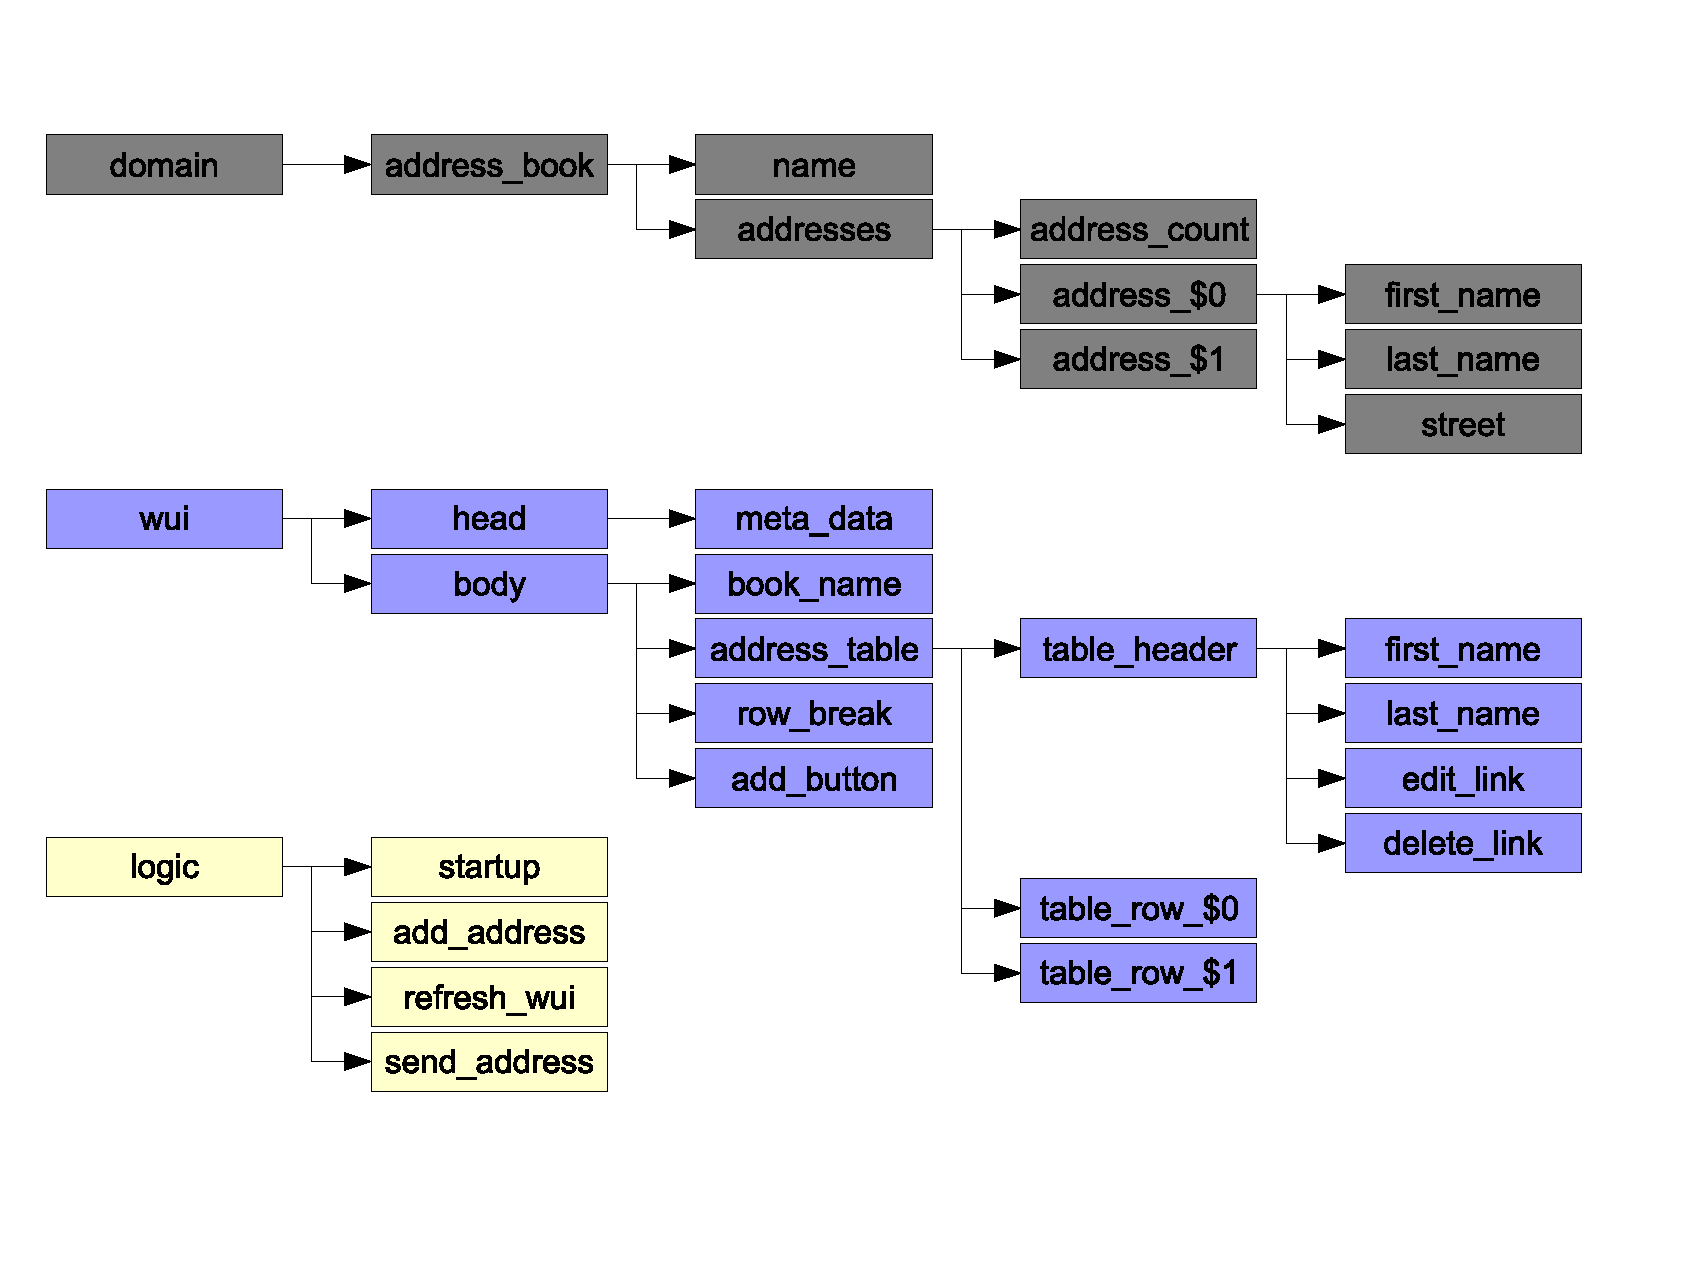
\includegraphics[scale=0.2]{vector/radesign.eps}
        \caption{ResAdmin Knowledge Models}
        \label{radesign_figure}
    \end{center}
\end{figure}

Due to the tremendous complexity of an \emph{Electronic Health Record} (EHR),
only a very small part of its data could be considered for the application
prototype. Administrative data like a person's name or address are standard
information found in all EHRs. A corresponding module named \emph{ResAdmin}
\cite{holzmueller2005} was therefore elected to be realised first. Its models
belong to three categories: \emph{Domain}, \emph{Web User Interface} (WUI) and
\emph{Logic} (figure \ref{radesign_figure}).

The addresses contained in the \emph{domain} branch of the knowledge tree are
manipulated across \emph{Hyper Text Markup Language} (HTML) \emph{User Interface}
(UI) models belonging to the \emph{web} branch of that same tree. An example
structure of a knowledge tree was shown in figure \ref{mvctree_figure}. Every
action model that a user can trigger through the WUI exists as part of the
\emph{logic} branch of the knowledge tree.

Independently of what kind of knowledge model (state or logic) was created,
ontological principles were strictly followed. Most importantly, relations
within a hierarchical model were always \emph{unidirectional}, that is from a
\emph{Whole-} to its \emph{Part} models, but never the other way around.
Additionally, however, logic models may reference and access runtime state
models.

Some of the logic models represent \emph{Translators} (compare section
\ref{communication_model_heading}). They extract address information
residing in the domain- and copy them to the web model, which is afterwards
sent to the human user as communication partner. This principle holds true for
the communication between application systems, only that then other than web
models are used as communication format. The vision to make all communication
channels really \emph{transparent} and easy to handle for the user now seems to
be coming true.



%
% $RCSfile: two_tier_architecture.tex,v $
%
% Copyright (c) 2001-2004. Christian Heller. All rights reserved.
%
% No copying, altering, distribution or any other actions concerning this
% document, except after explicit permission by the author!
% At some later point in time, this document is planned to be put under
% the GNU FDL license. For now, _everything_ is _restricted_ by the author.
%
% http://www.cybop.net
% - Cybernetics Oriented Programming -
%
% http://www.resmedicinae.org
% - Information in Medicine -
%
% @author Christian Heller <christian.heller@tuxtax.de>
%

\subsection{Two Tier Architecture}
\label{two_tier_architecture_heading}

The proposed CYBOP communication architecture is currently implemented in form
of a \emph{Two-Tier} architecture (figure \ref{two_tier_architecture_figure}).

\begin{figure}[ht]
    \begin{center}
       \includegraphics[scale=0.4]{vector/two_tier_architecture.eps}
       \caption{Two Tier Architecture}
       \label{two_tier_architecture_figure}
    \end{center}
\end{figure}

It shows how two autarchic components (Application A and B) intercommunicate and
save their domain data in different ways. Each component fulfills a special task
and works as a client as well as a server. One can recognize the two patterns
\emph{DataMapper} and \emph{DTO}.\\
If a client requests some data from another component, the central object
\emph{DataTransferTranslator} collects all needed information from the
\emph{DomainModel} and encodes (packs) them into one \emph{DataTransferModel}.
Now, the \emph{Server} object can send this \emph{DTO} back to the requesting
client component. On the other side of the wire, the \emph{Client} object receives
the \emph{DTO}, a \emph{DataTransferTranslator} decodes (unpacks) the data and
writes them into the \emph{DomainModel}.\\
In this example, the two components are located on the same host. It is also
possible to distribute them. Therefore, each component is also able to communicate
with other components that are situated somewhere in the network. The arrows in
applications indicate the dependencies between the single architectural elements,
whereas the outside arrows show the communication between components and database
server.\\
All data storing operations are hidden in a special \emph{PersistenceTranslator}
like the one shown in figure \ref{two_tier_architecture_figure}, on the example
of a database. The SQL statements were placed in a separate package. If there is
the need for getting information from a database, the translator uses the statements
of the \emph{SQL Package} and maps data of the result set to the \emph{DomainModel}.


%
% $RCSfile: three_tier_architecture.tex,v $
%
% Copyright (c) 2001-2004. Christian Heller. All rights reserved.
%
% No copying, altering, distribution or any other actions concerning this
% document, except after explicit permission by the author!
% At some later point in time, this document is planned to be put under
% the GNU FDL license. For now, _everything_ is _restricted_ by the author.
%
% http://www.cybop.net
% - Cybernetics Oriented Programming -
%
% http://www.resmedicinae.org
% - Information in Medicine -
%
% @author Christian Heller <christian.heller@tuxtax.de>
%

\subsection{Three Tier Architecture}
\label{three_tier_architecture_heading}

To provide a more comfortable structure than the typical \emph{Two-Tier}
architecture as shown in section \ref{two_tier_architecture_heading}, there is
the necessity of a \emph{Three-} or \emph{Multi-Tier} Architecture.
If, for example, the location of the database server was changed then, in a
\emph{Two-Tier} architecture, all clients would have to be updated.
Figure \ref{three_tier_architecture_figure} makes a proposition to solve
this problem.

\begin{figure}[ht]
    \begin{center}
       \includegraphics[scale=0.45]{vector/three_tier_architecture.eps}
       \caption{Three Tier Architecture}
       \label{three_tier_architecture_figure}
    \end{center}
\end{figure}



